\chapter{Caso de Estudio}
\label{chapter:chapter4}
\section{Generador de Perfiles Energéticos}
El uso de los vehículos es particular al estilo de vida de cada usuario, tanto para vehículos de
combustión como para vehículos eléctricos. Por ello, es necesario generar perfiles energéticos que
sinteticen y agrupen los diferentes usos energéticos — y por tanto la necesidad de carga de dichos
vehículos — de los usuarios.\\

En el primer bloque que compone el trabajo, se ha desarrollado un algoritmo generador de perfiles 
de carga de EVs, partiendo del \textit{Electric Vehicle Charging Dataset}~\cite{kaggle_ev_charging_patterns}.
A partir de este dataset, se han generado nuevas muestras sintéticas de perfiles de carga y uso 
típico de las estaciones de carga. Para ello, se ha utilizado una de las herramientas de IA 
Generativa, presentada en el Capítulo~\ref{chapter:chapter2}, concretamente se ha hecho uso de una
GAN.\\

Los parámetros de la GAN se han ajustado para que los perfiles generados representen adecuadamente
la variabilidad de la demanda energética para la carga de un EV, teniendo en cuenta las restricciones,
requisitos y hábitos del usuario. El resultado es un conjunto de perfiles energéticos que pueden
ser utilizados para entrenar y evaluar el gestor de carga de EVs, así como para simular diferentes
escenarios de carga y consumo energético.\\

A partir de los datos obtenidos, tanto del dataset original como los generados, se han podido 
extraer una serie de perfiles y patrones de consumo energético, que se han agrupado en distintas 
categorías, y que se han utilizado para entrenar el gestor de carga de EVs. Estos perfiles se han
usado principalmente para ofrecer al gestor un rango de disponibilidad de carga del vehículo y 
oportunidades de carga a lo largo del día, en funcion de la "personalidad" de cada uno de los 
usuarios.\\

Es importante resaltar que, con el fin de introducir algo de variabilidad en los perfiles, y reducir
el determinismo en cuanto a la disponibilidad de carga se refiere, durante el proyecto se ha 
tratado esta funcion de disponibilidad como una función probabilística definida a trozos. Esto 
significa que, para cada perfil de usuario, según la hora del día, se ha asignado una probabilidad
de que el usuario esté disponible para cargar su vehículo eléctrico. El número concreto de esta
probabilidad asignada, se ha obtenido juntando la la información del dataset original, la 
información obtenida de los datos generados, y la idea general detrás de cada perfil de usuario, y
sus características más convencionales.\\

Los perfiles generados se han agrupado en las siguientes categorías, que representan los
distintos tipos de usuarios y sus hábitos de carga:
\begin{table}[H]
    \centering
    \begin{tabular}{p{2cm} p{7.25cm} p{2.5cm} p{1.25cm}}
        \toprule
        \textbf{Perfil} & \textbf{Hábitos de carga} & \textbf{Horas} & \textbf{Prob.} \\
        \midrule
        Trabajador (\texttt{worker}) &
        Carga principalmente de noche; baja disponibilidad en horario laboral. &
        00:00–06:00 \newline 06:00–21:00 \newline 21:00–00:00 &
        0.95 \newline 0.10 \newline 0.85 \\
        \addlinespace[0.5ex]
        Flexible &
        Disponibilidad media y estable, con ligera bajada en horario laboral. &
        00:00–08:00 \newline 08:00–18:00 \newline 18:00–00:00 &
        0.80 \newline 0.60 \newline 0.75 \\
        \addlinespace[0.5ex]
        Jubilado (\texttt{retired}) &
        Alta disponibilidad todo el día, salvo ausencias puntuales a mediodía y tarde. &
        00:00–12:00 \newline 12:00–16:00 \newline 16:00–00:00 &
        0.95 \newline 0.70 \newline 0.90 \\
        \addlinespace[0.5ex]
        Viajero (\texttt{traveller}) &
        Alta disponibilidad salvo ausencias frecuentes en horario diurno y algunas tardes. &
        00:00–08:00 \newline 08:00–18:00 \newline 18:00–00:00 &
        0.90 \newline 0.40 \newline 0.80 \\
        \addlinespace[0.5ex]
        Nocturno (\texttt{night\_owl}) &
        Carga casi exclusiva por la noche; baja disponibilidad diurna. &
        00:00–06:00 \newline 06:00–20:00 \newline 20:00–00:00 &
        0.98 \newline 0.15 \newline 0.90 \\
        \bottomrule
    \end{tabular}
    \caption{Perfiles energéticos generados para usuarios de EV, horas y probabilidades de disponibilidad}
\end{table}

\section{Precios de la Electricidad}
Para el desarrollo del trabajo son esenciales los precios de la electricidad, que se han obtenido
directamente de Red Eléctrica de España (REE)~\cite{pvpc_csv_2024}. Se han escogido los precios de 
la electricidad para la península ibérica (PVPC) para el año 2021, ya que es muy reciente, está
completo y coincide con los datos generado con LPG. A continuación se muestra un análisis de los 
precios durante dicho año:
\begin{figure}[H]
    \centering
    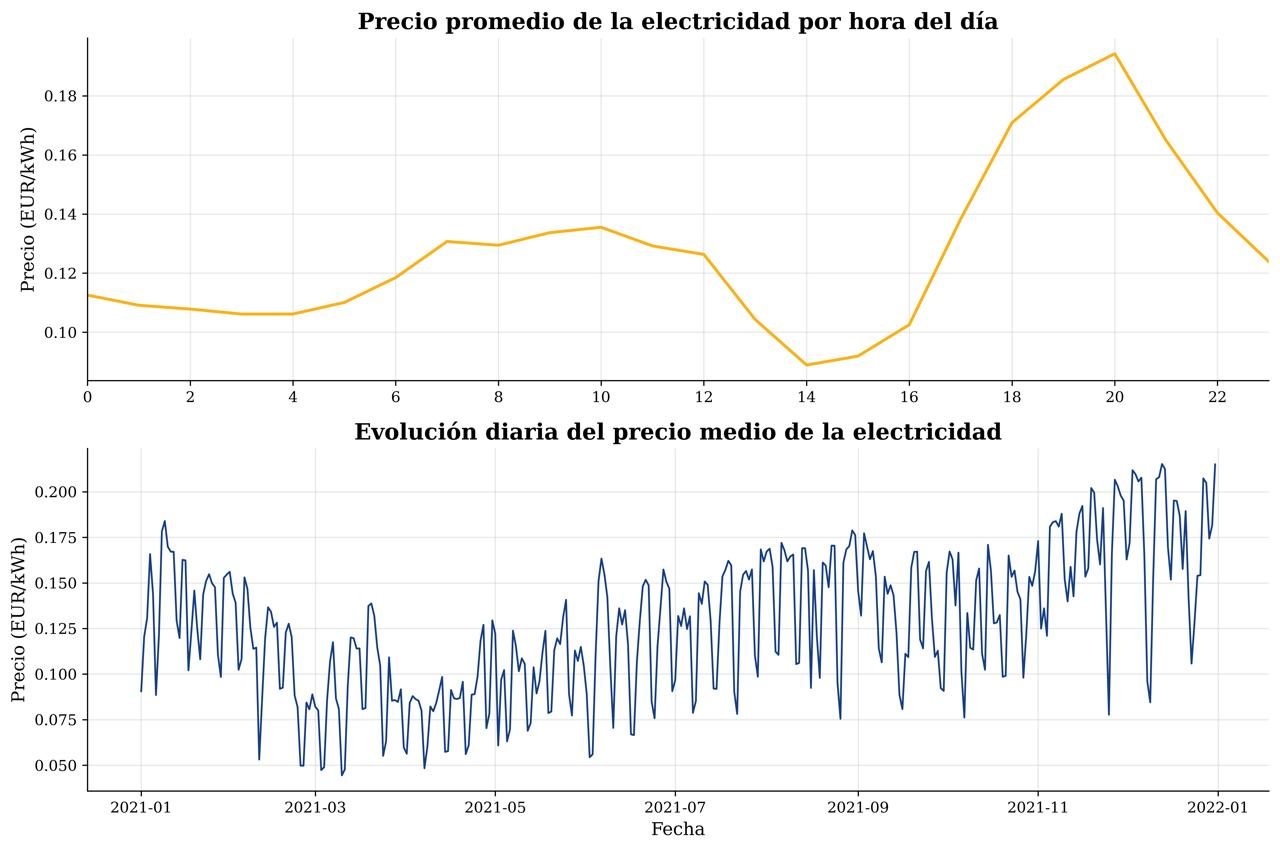
\includegraphics[width=0.65\textwidth]{images/preciosElectricidad.jpg}
    \caption{Precios de la electricidad en España durante el año 2021. Fuente: Elaboración propia a partir de datos de REE.}
    \label{fig:precios_electricidad}
\end{figure}

\section{Generador de Consumo}
Este segundo bloque se centra en la tarea de generación de consumos energéticos domésticos,
utilizando el software \textit{Load Profile Generator (LPG)}. Se ha configurado una vivienda de
tipo unifamiliar en el entorno urbano de Madrid, modelada para representar una situación típica
de un hogar con presencia de vehículo eléctrico, hijos y hábitos laborales estándar. La configuración
empleada es la siguiente:

\begin{table}[H]
    \centering
    \begin{tabular}{p{4cm} p{9.8cm}}
        \\[-1.5ex] % Espacio extra antes de la primera fila
        \toprule
        \textbf{Parámetro} & \textbf{Descripción} \\
        \midrule
        Tiempo simulado & 365 días (1 año completo) \\
        \\[-1.5ex]
        Resolución temporal interna & 1 minuto \\
        \\[-1.5ex]
        Resolución temporal externa & 15 minutos \\
        \\[-1.5ex]
        Ubicación geográfica & Madrid, España \\
        \\[-1.5ex]
        Tipo de vivienda & Unifamiliar, tamaño medio (100–150 m\textsuperscript{2}), con garaje y trastero \\
        \\[-1.5ex]
        Aislamiento térmico & Estándar \\
        \\[-1.5ex]
        Equipamiento & Completo en electrodomésticos \\
        \\[-1.5ex]
        Composición familiar &
        \begin{itemize}[noitemsep, topsep=-10pt]
            \item Mujer (trabaja fuera, jornada completa)
            \item Hombre (trabaja en casa, jornada parcial)
            \item Niños: uno en edad escolar, otro en edad preescolar
        \end{itemize} \\
        \\[-1.5ex]
        Vehículo eléctrico &
        \begin{itemize}[noitemsep, topsep=-10pt]
            \item Un coche compartido
            \item Uso diario laboral y escolar
            \item Carga preferente nocturna
        \end{itemize} \\
        \\[-1.5ex]
        Perfil de temperatura & Datos realistas para 2025 en Madrid \\
        \\[-1.5ex]
        Calendario & Incluye fines de semana y festivos nacionales \\
        \bottomrule
    \end{tabular}
    \caption{Parámetros de configuración de la vivienda en LPG}
\end{table}
La vivienda, como se muestra en la anterior tabla, está ocupada por cuatro personas, cuyas rutinas 
diarias han sido configuradas para representar un hogar realista con uso intensivo de energía:

\begin{itemize}
    \item \textbf{Adulto 1 (mujer):} trabaja fuera del hogar a jornada completa (8h–17h),
    desplazándose en vehículo eléctrico cinco días a la semana. Contribuye a la carga del
    EV en horario nocturno.

    \item \textbf{Adulto 2 (hombre):} trabaja parcialmente desde casa, con jornada reducida.
    Su presencia en el hogar durante el día impacta en el uso de climatización, cocina y
    dispositivos electrónicos.

    \item \textbf{Niño 1:} escolarizado, con jornada matinal completa. Genera picos de consumo
    por la mañana y por la tarde (actividades, ducha, iluminación).

    \item \textbf{Niño 2:} edad preescolar, cuidado en casa. Su presencia constante condiciona
    el uso continuo de climatización, iluminación y aparatos electrónicos de ocio.
\end{itemize}
Con estas características cargadas en la configuración del programa generador, se ha procedido a la
generación de los siguientes datos de consumo energético:

\begin{table}[H]
\centering
    \begin{tabular}{@{}p{3.4cm} p{10.6cm}@{}}
        \toprule
        \textbf{Categoría} & \textbf{Descripción} \\
        \midrule
        Electrodomésticos de cocina &
        Horno, vitrocerámica, microondas; lavavajillas; frigorífico y congelador (consumo continuo) \\
        \\[-1.5ex]
        Electrodomésticos de limpieza & Lavadora, secadora y aspiradora \\
        \\[-1.5ex]
        Entretenimiento y oficina &
        Televisores, ordenadores, router; consolas, altavoces, impresoras \\
        \\[-1.5ex]
        Iluminación &
        Luz general por estancias, activación dependiente de presencia y hora del día \\
        \\[-1.5ex]
        Climatización &
        Calefacción eléctrica (invierno); aire acondicionado o ventiladores (verano) \\
        \\[-1.5ex]
        Agua caliente sanitaria (ACS) &
        Consumo eléctrico en ausencia de caldera de gas \\
        \\[-1.5ex]
        Carga del vehículo eléctrico &
        Carga según trayectos diarios; horarios preferentes nocturnos \\
        \\[-1.5ex]
        Consumo en espera (stand-by) &
        Dispositivos conectados permanentemente; carga latente (TV, router, cargadores)\\
        \bottomrule
    \end{tabular}
\caption{Categorías de consumo energético simuladas}
\end{table}
Con esta configuración se han generado los consumos energéticos horarios agregados para los 
distintos elementos. Este perfil de consumo no gestionable sirve como input para el gestor 
inteligente de carga, presentado en la siguiente sección.

\subsubsection{Descripción de los Datos Generados}
A continuación se muestran algunas de las gráficas generadas por la aplicación, que describen los datos generados
por el LPG. Estas gráficas muestran el consumo energético de la vivienda a lo largo de un año,
con una resolución de 15 minutos.
\begin{figure}[H]
    \centering
    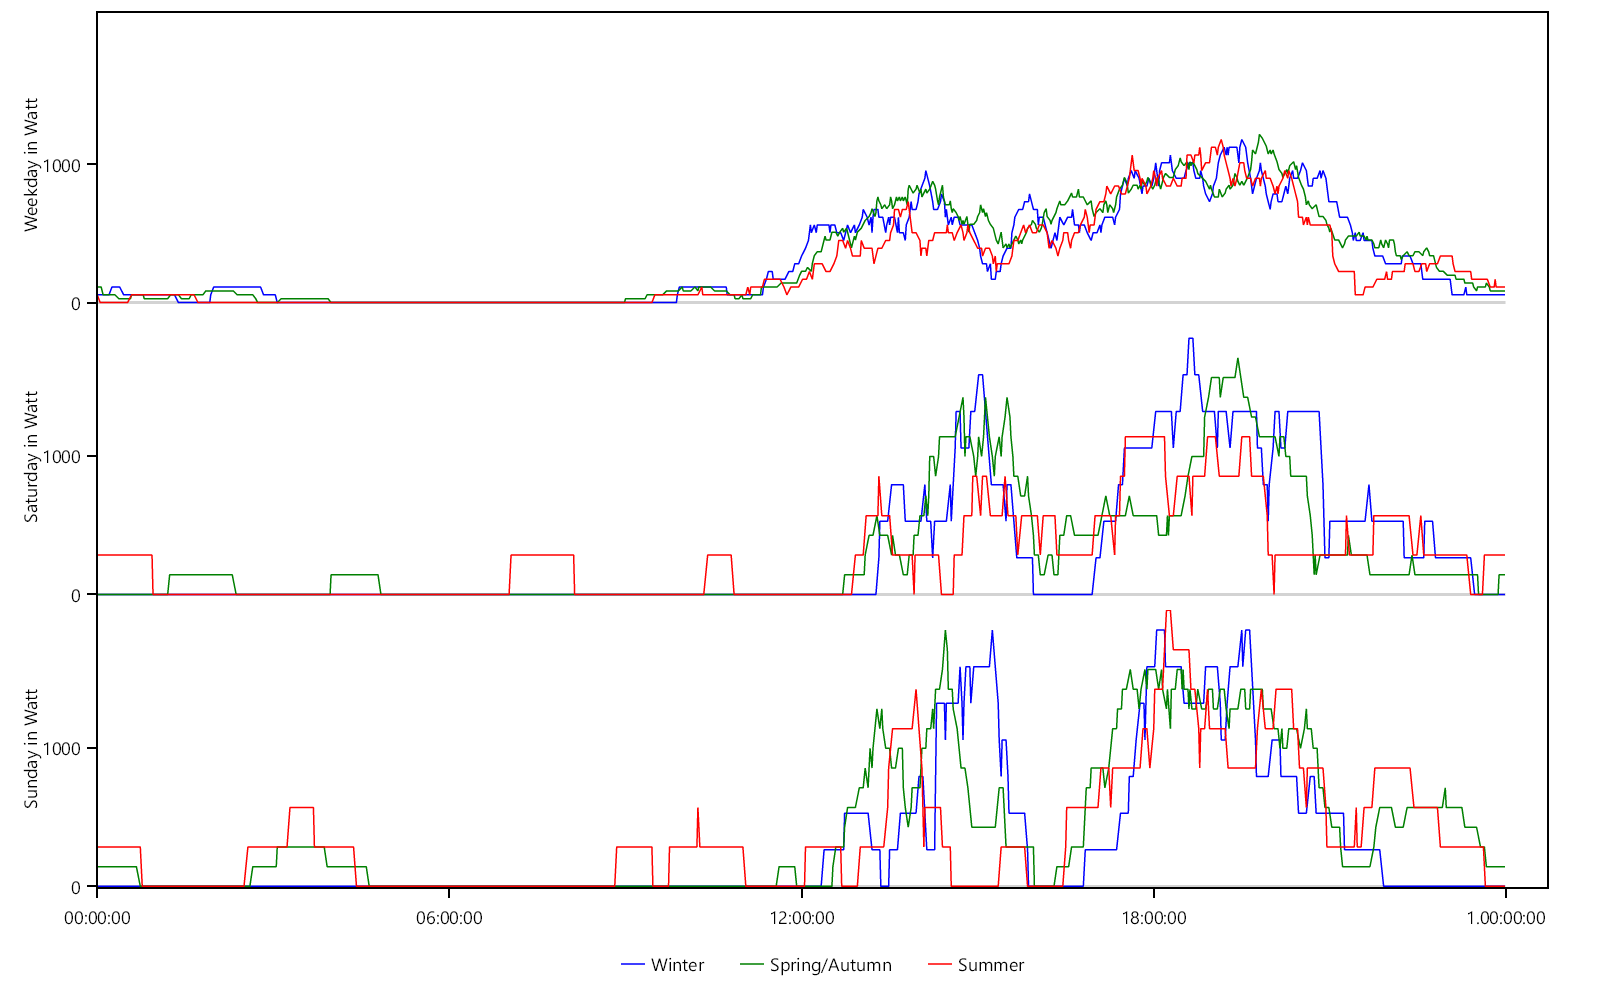
\includegraphics[width=0.4957\textwidth]{images/LPG/WeekdayProfiles.Electricity for Car Charging.png}
    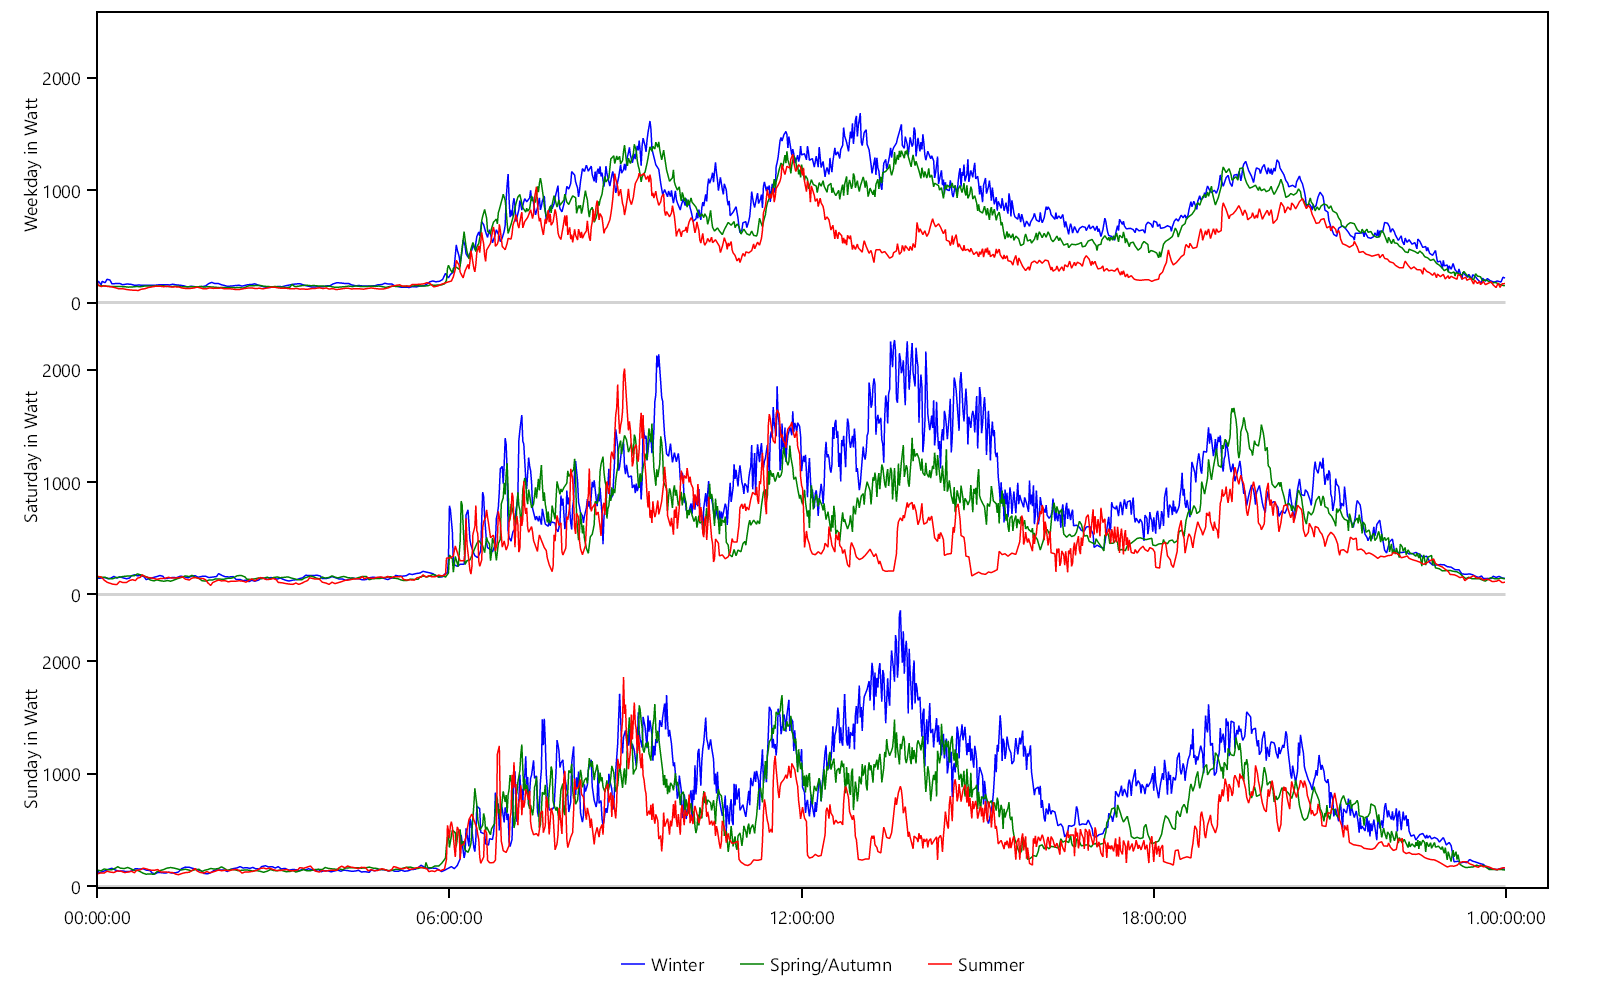
\includegraphics[width=0.4957\textwidth]{images/LPG/WeekdayProfiles.Electricity.png}
    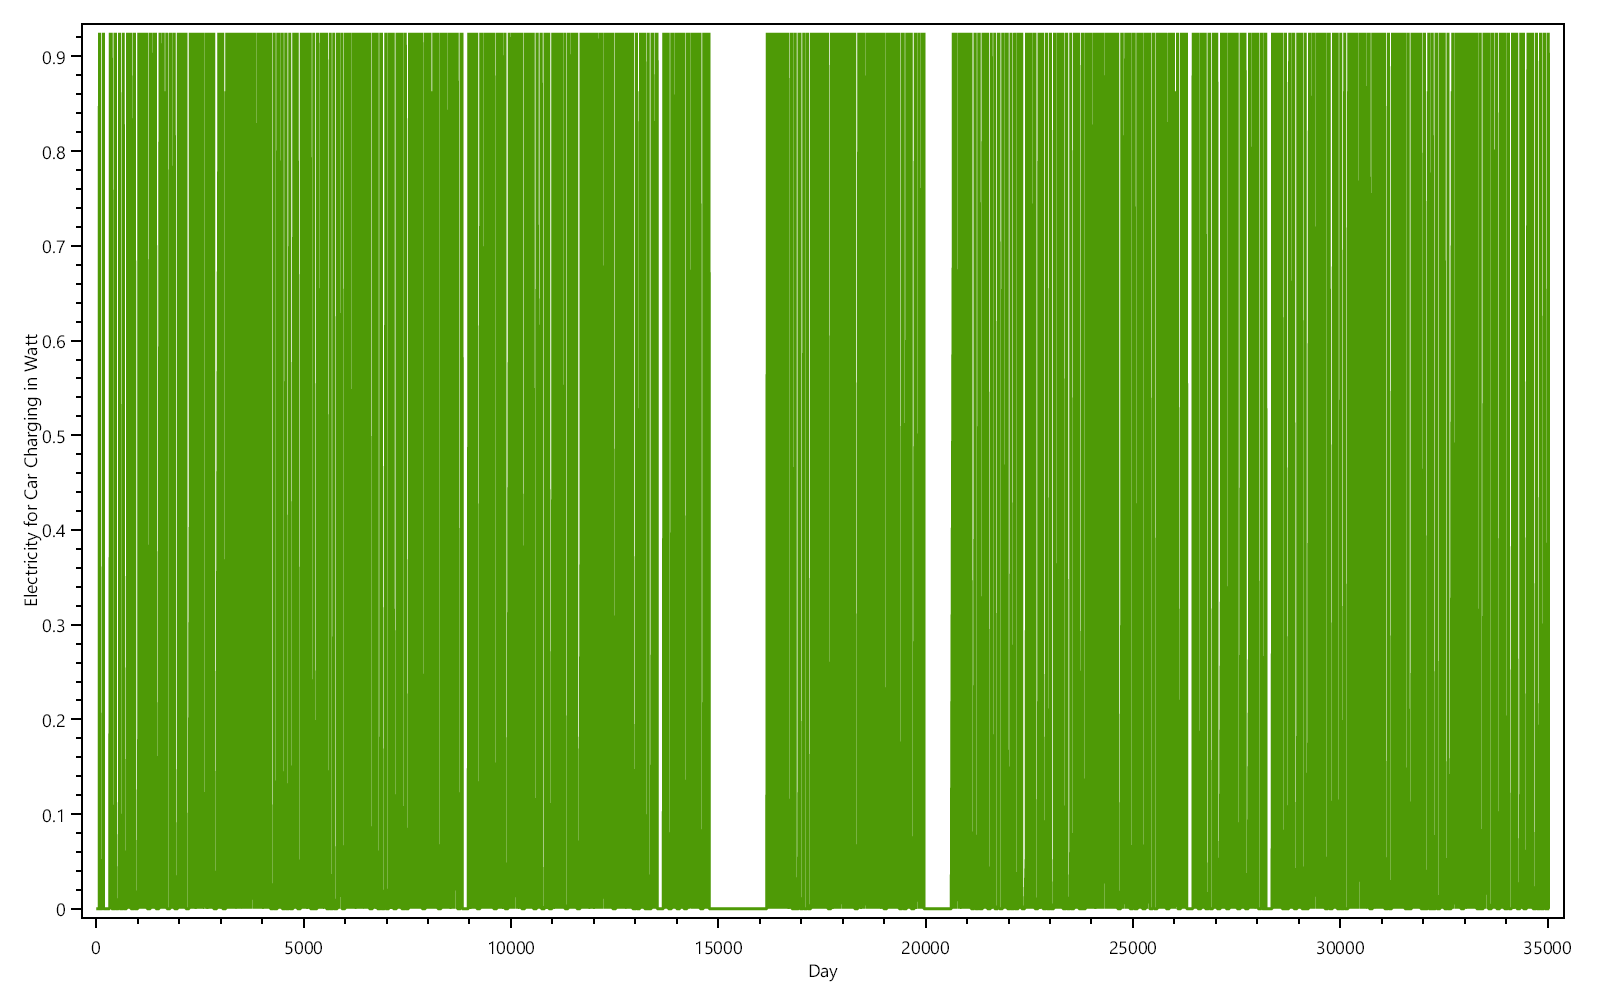
\includegraphics[width=0.4957\textwidth]{images/LPG/SumProfiles_900s.Electricity for Car Charging.png}
    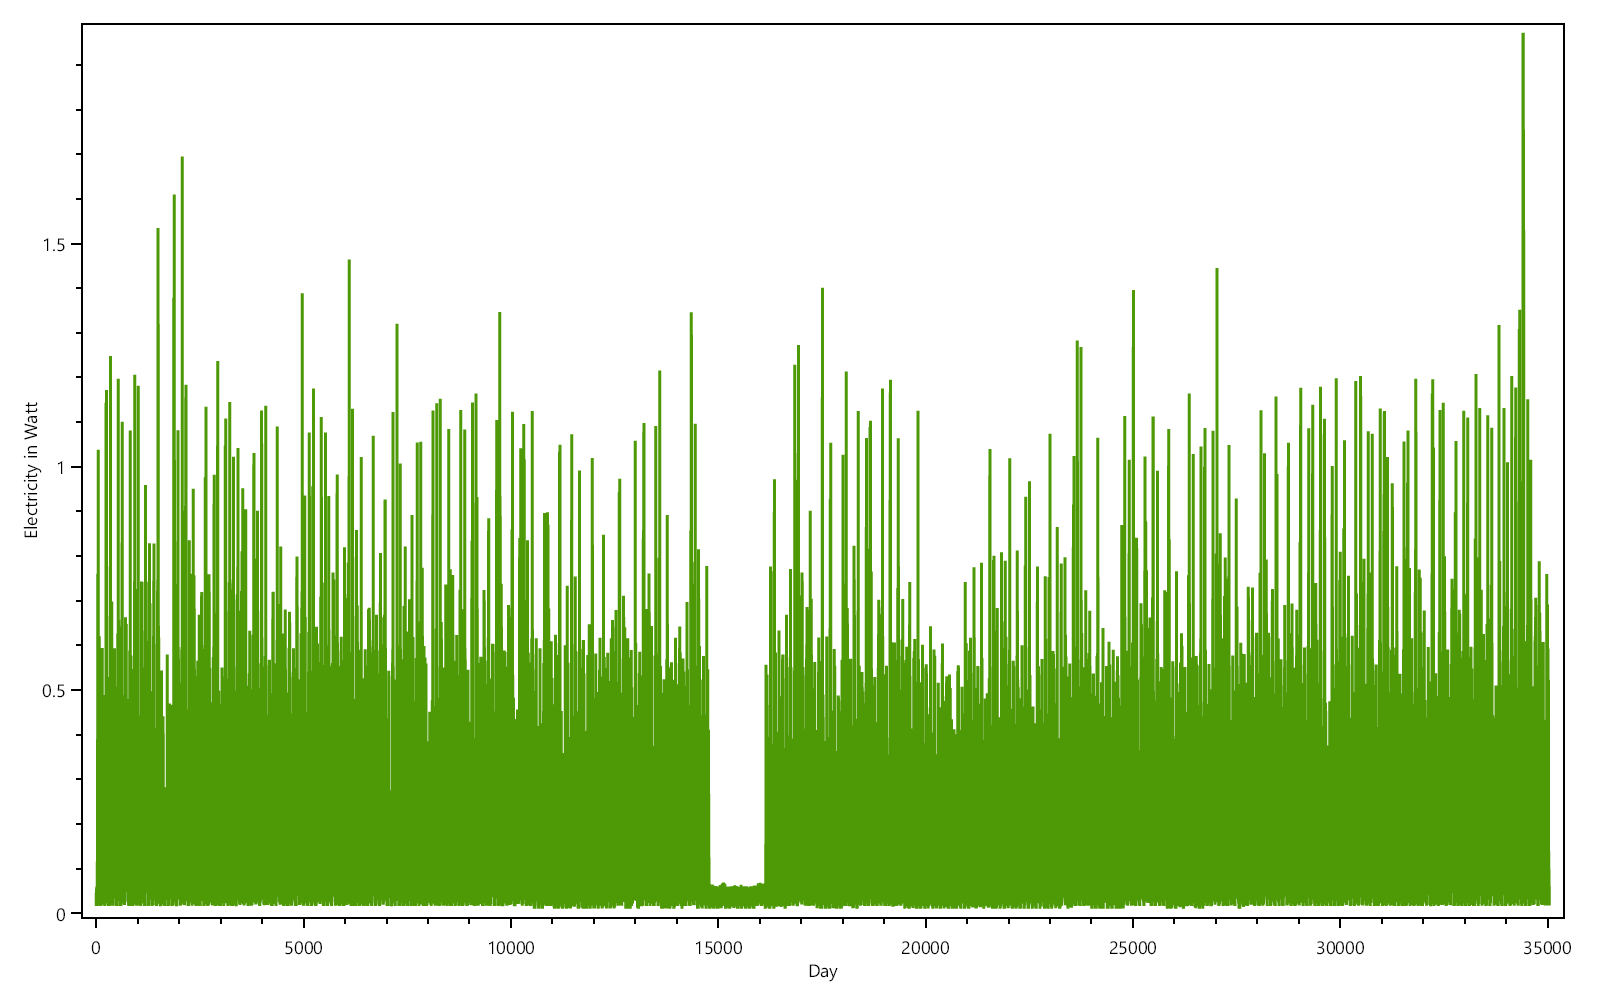
\includegraphics[width=0.4957\textwidth]{images/LPG/SumProfiles_900s.Electricity.png}
    \caption{Gráficas generadas por el LPG.}
    \label{fig:lpg_consumo}
\end{figure}

Las dos primeras gráficas muestran el consumo energético de la vivienda, promediado a lo largo de 
un año, durante los días laborables de la semana y el fin de semana. La gráfica de la izquierda 
muestra el consumo energético para la carga del vehículo eléctrico, mientras que la gráfica de la 
derecha muestra el consumo total de energía de la vivienda. Además, se han representado las 
distintas estaciones del año con líneas de distinto color, para un análisis más detallado.\\

Las gráficas en la fila inferior muestran el consumo total de energía para la carga del EV, y en
general a lo largo del año, respectivamente. Se puede observar que el consumo energético varía a lo 
largo del año, con picos de consumo en invierno y verano, y una tendencia general de aumento del 
consumo a lo largo del año.\\

Estas gráficas, siendo una muestra de todas las disponibles para el análisis, proporcionan una 
visión general del consumo energético de la vivienda, y son útiles para entender los patrones de
consumo y carga del vehículo eléctrico. Además, permiten identificar los momentos de mayor
consumo energético, lo que es esencial para la gestión eficiente de la carga del EV.\\

Más imágenes de las gráficas generadas por el LPG, y análisis propios, se pueden encontrar en el
anexo~\ref{appendix:appendixA}.

\section{Gestor de Carga de EVs}
El gestor de carga es el tercer y último bloque del trabajo, y es realmente el foco del mismo. 
Para su desarrollo, se ha implementado una red neuronal de aprendizaje por refuerzo DQN añadiendo 
unas capas de LSTM, que se ha entrenado con los perfiles de consumo energético, obtenidos tras la 
generación de datos adicionales; y toda la información de la vivienda y del vehículo eléctrico.\\

El gestor de carga tiene como objetivo optimizar la carga del vehículo eléctrico, minimizando por 
supuesto el coste incurrido en la carga, teniendo en cuenta las restricciones y requisitos del usuario. 
Para ello, se ha implementado un algoritmo de aprendizaje por refuerzo, que permite al gestor de carga 
aprender de la experiencia y mejorar su rendimiento a lo largo del tiempo.\\

Antes de usar redes neuronales, se ha implementado un algoritmo de optimización clásico, que
sirve como base para comparar el rendimiento del gestor de carga. Este algoritmo utiliza las 
técnicas de optimización clásica, tal y como se ha presentado en el Capítulo~\ref{chapter:chapter2}, 
para obtener una solución óptima al problema que presenta la carga del EV.\\

\subsection{Optimización Clásica}
Primeramente, se han de definir el conjunto de variables que después formarán las restricciones y
objetivos del problema de optimización. En este caso, las variables son las siguientes:
\begin{itemize}
    \item $\mathit{P}(t)$: Potencia en el instante $t$ [kW]
    \item $\mathit{E}(t)$: Energía en el instante $t$ [kWh]
    \item $P_\text{Max}$: Potencia máxima en el cargador [kW]
    \item $\mathit{SOC}(t)$: Estado de carga en el instante $t$ [kWh]
    \item $P_{NG}(t)$: Potencia del No Gestionable en $t$ [kW]
    \item $\eta$: Eficiencia del sistema
    \item $A(t)$: Disponibilidad en el instante $t$ [1: disponible, 0: no]
    \item $p(t)$: Precio de la electricidad en el instante $t$ [€/kWh]
    \item $C(t)$: Coste de carga en el instante $t$ [€]
\end{itemize}

Una vez se tienen claras las variables, tras un análisis del problema, se definen las siguientes
restricciones y función objetivo:
\begin{alignat}{3}
    \min_{P(t)} \quad & \sum_{t} C(t) = \sum_{t} E(t) \cdot p(t) && \\
    \text{s.a.} \quad 
    & 0 \leq P(t) \leq P_{\text{max}} \cdot A(t) && \qquad \forall t \\
    & P(t) + P_{\text{NG}}(t) \leq P_{\text{red}} && \qquad \forall t \\
    & SOC(t+1) = SOC(t) + \eta \cdot \frac{P(t) \cdot \Delta t}{\text{capacidad}} && \qquad \forall t \\
    & \sum_{t} P(t) \cdot \Delta t \geq (SOC_f - SOC_i) \cdot \text{capacidad} &&
\end{alignat}
 
Una vez ya se ha planteado el problema, se implementa el Python~\cite{python2024language}
usando la librería \textit{Pyomo}~\cite{pyomo2024} para definir el modelo de optimización, y
\textit{GurobiPy}~\cite{gurobi2024} como solver. El código se ha implementado de forma que se pueda
cargar el perfil de consumo energético generado por el LPG, y se pueda ejecutar el algoritmo de
optimización para obtener la solución óptima al problema de carga del EV.\\

Los resultados obtenidos con este algoritmo de optimización clásico sirven como base para
comparar el rendimiento del gestor de carga basado en aprendizaje por refuerzo, y para evaluar la
mejora en la eficiencia y reducción de costes que se puede lograr con el uso de técnicas del RL.\\ 

En la Figura~\ref{fig: classic_daily_profiles} se muestra el comportamiento diario del algoritmo de
optimización clásico para el perfil \texttt{worker}, donde se observa la evolución de la potencia
entregada al cargador y la evolución del estado de carga (SOC) del vehículo eléctrico a lo largo 
del día. Por otro lado, en la Figura~\ref{fig: classic_global_profiles} se muestran las mismas 
variables pero a lo largo de un mes entero, donde se puede observar las tendencuas de carga y
consumo del vehículo eléctrico, así como la variabilidad en la potencia aplicada y el SOC a lo largo
del mes.
\begin{figure}[H]
    \centering
    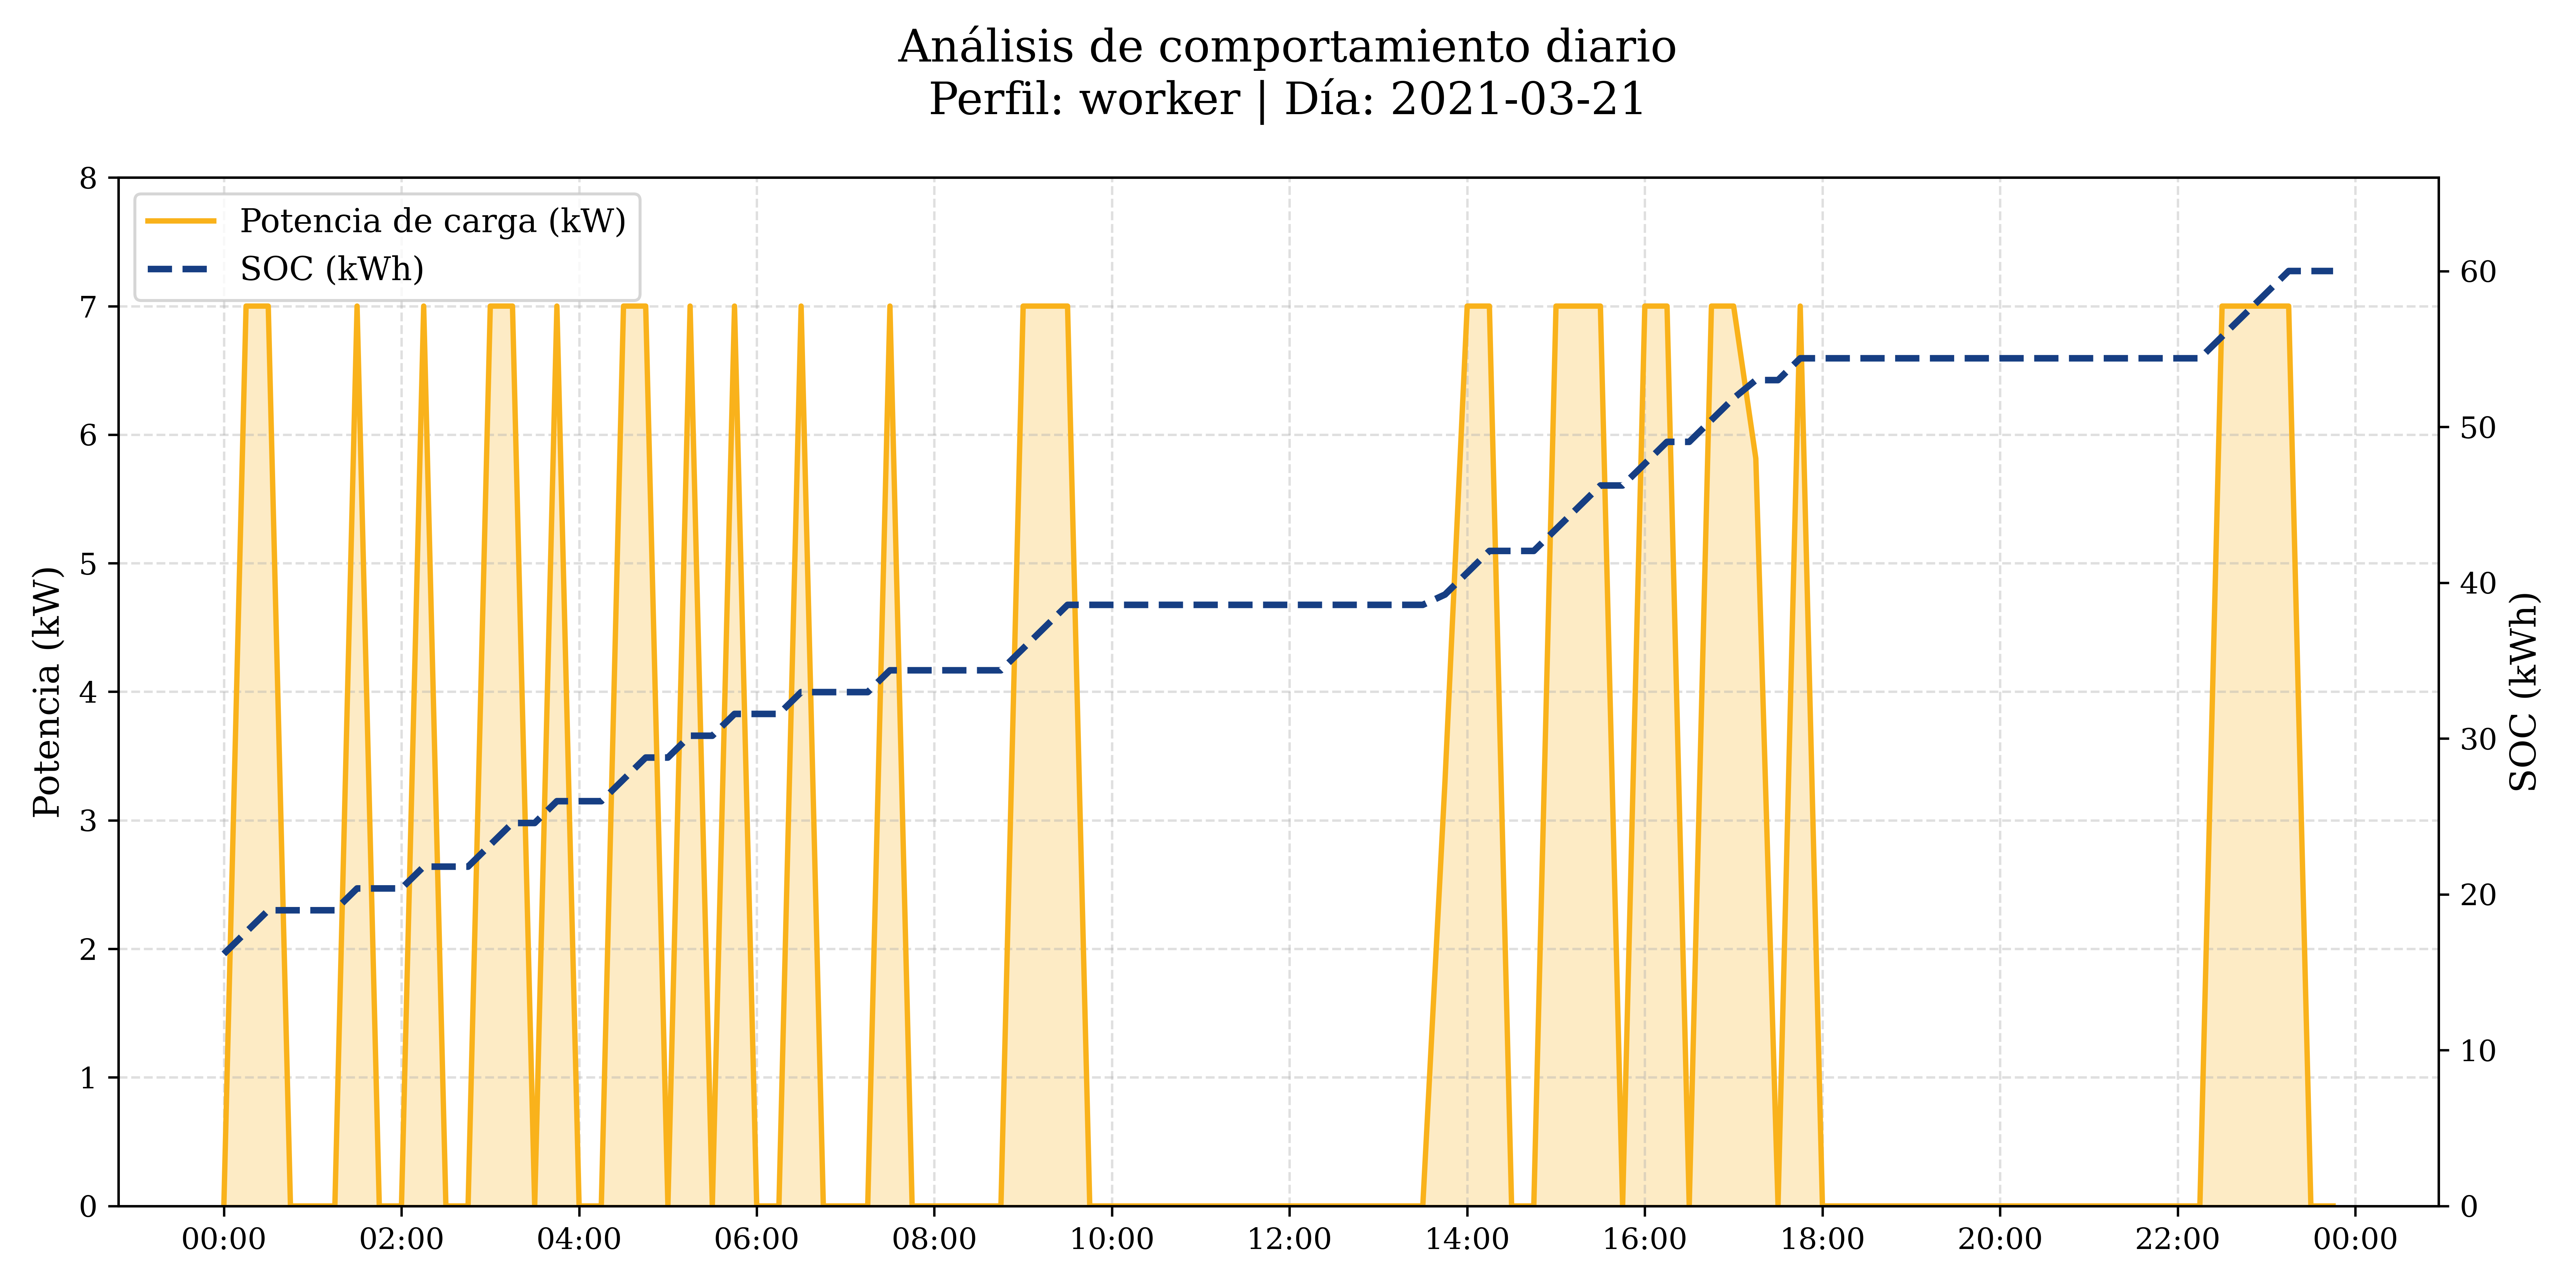
\includegraphics[width=0.7\textwidth]{images/classic/daily_behavior_2021-03-21_worker.png}
    \caption{Resultados del algoritmo de optimización clásico para el perfil \texttt{worker}: 
    potencia aplicada y evolución del SOC en un día. Fuente: Elaboración propia.}
    \label{fig: classic_daily_profiles}
\end{figure}
\begin{figure}[H]
    \centering
    \includegraphics[width=0.7\textwidth]{images/classic/global_july_classic_worker.png}
    \caption{Resultados del algoritmo de optimización clásico para el perfil \texttt{worker}: 
    potencia aplicada y evolución del SOC a lo largo de un mes. Fuente: Elaboración propia.}
    \label{fig: classic_global_profiles}
\end{figure}

En el análisis diario, se puede observar cómo el algoritmo de optimización clásico se adapta a las
costumbres impuestas por el perfil de usuario, cargando mayoritariamente el EV durante la noche, y
en momentos del día en los que el consumo energético es menor, y hay mayor probabilidad de que el 
vehículo esté disponible para la carga. Además, se observa que el SOC del vehículo se mantiene
dentro de los límites establecidos, y se carga de forma eficiente para minimizar el coste total de
la carga.\\

Durante el análisis mensual, la tendencia de carga del EV para este perfil se mantiene, cargando
principalmente pronto durante la noche. Ocurre una cosa curiosa en el mes de julio en estos 
resultados en particular, y es que el algoritmo no consigue encontrar una solución óptima para
la carga del EV sobre el día 14 del mes.\\

El mes representado no ha sido seleccionado de forma aleatoria, sino que se ha escogido un mes en 
el que se puede observar uno de los principales riesgos de la gestión de la carga de EVs con un
algoritmo de optimización clásico, y es que, si el perfil de consumo energético es muy variable,
las condciones del EV cambian, o hay un cambio inesperado en cualquier campo, el algoritmo
de optimización clásico no es capaz de adaptarse a esos cambios, y por tanto no consigue encontrar
una solución óptima. Esto es un problema importante, ya que en la vida real, si el usuario se 
encunetra en una situación similar, se encontraría completamente desprotegido y su vehículo sin
cargar.\\

Se muestra únicamente el perfil \texttt{worker} como ejemplo más representativo, ya que sería el
perfil de consumo energético más habitual. Los resultados y visualizaciones adicionales tanto para
este perfil como para los demás se pueden encontrar en el anexo~\ref{appendix:appendixA}.\\

Siguiendo con los resultados de la optimización clásica, a continuación se presentan una serie de
métricas y resultados adicionales obtenidos por el algoritmo de optimización clásico, que
permiten evaluar su rendimiento y eficiencia en la gestión de la carga del vehículo eléctrico.
\begin{table}[H]
    \centering
    \begin{tabular}{lccc}
        \textbf{Perfil} & $\overline{\text{Coste}}$ (EUR) & $\overline{\text{Energía}}$ (kWh) & Eficiencia(kWh/EUR) \\
        \midrule
        retired & 27.14  & 244.08 & 8.99 \\
        night\_owl & 27.57  & 244.53 & 8.87 \\
        flexible & 27.69  & 245.02 & 8.85 \\
        traveller & 27.23  & 242.74 & 8.92 \\
        worker & 27.35  & 244.08 & 8.92 \\
        \bottomrule
    \end{tabular}
    \caption{Resumen de métricas diarias por perfil para la optimización clásica.}
    \label{tab:metrics_opt_classic_aligned}
\end{table}

En primer lugar, se puede apreciar la tremenda similitud entre los resultados obtenidos
para los distintos perfiles de usuario, ya que todos ellos tienen un comportamiento muy similar
en cuanto a la carga del vehículo eléctrico, aunque los perfiles son tremendamente distintos.\\

Para empezar, el coste medio diario de la carga. Los valores obtenidos, siguiendo la tónica del 
optimizador, se mantienen muy estables, con un coste total de carga de alrededor de 27.3 EUR por 
día, con una eficiencia de carga de alrededor de 8.9 kWh por EUR. Esto indica que el algoritmo de 
optimización clásico es capaz de gestionar la carga del vehículo eléctrico de forma eficiente, 
minimizando el coste total de la carga, y adaptándose a las condiciones del mercado eléctrico y a 
las restricciones del usuario.\\

Además, la nergía media diaria cargada consigue mantener esta estabilidad a lo largo de los 
distintos perfiles estudiados, con un valor medio de alrededor de 244 kWh por día. Naturalmente, por 
cómo se ha modelado la batería del EV al principio de cada día, introduciendo una variabilidad
aleatoria entre 3\% y 25\% de SOC, se puede observar que la energía total cargada varía ligeramente 
entre los perfiles, pero se mantiene en un rango muy similar, al durar el estudio un año completo.\\

Finalmente, la métrica llamada \textit{eficiencia} se ha calculado como la relación entre la energía
cargada y el coste total de la carga, y se ha mantenido en torno a 8.9 kWh por EUR a lo largo de 
todos los perfiles. Esta métrica es muy importante, ya que indica la eficiencia del algoritmo de 
optimización clásico en la gestión de la carga del vehículo eléctrico, y su capacidad para 
minimizar el coste total de la carga, al mismo tiempo que se asegura de que el vehículo esté
cargado adecuadamente para cada situación.\\

Por último, se han registrado los tiempos de ejecución del algoritmo de optimización clásica, tanto 
para la resolución de cada perfil de usuario de forma individual como para el conjunto completo de 
perfiles. Los resultados obtenidos son los siguientes:
\begin{itemize}
    \item \textbf{Tiempo acumulado resolviendo modelos individuales:} 0.57 segundos
    \item \textbf{Tiempo total de optimización:} 8.05 segundos
\end{itemize}

Estos valores reflejan la eficiencia computacional del enfoque clásico, permitiendo resolver el 
problema de optimización en tiempos muy reducidos incluso para múltiples perfiles.

\subsection{Red Neuronal de Aprendizaje por Refuerzo}
Para la implementación del gestor, se ha usado una red neuronal de aprendizaje por refuerzo DQN-LSTM, 
entrenada con los mismos datos que el algoritmo de optimización clásico, es decir, los perfiles de
consumo energético generados por el LPG, y la información de la vivienda y del vehículo eléctrico. 
En cierta forma, tal y como se ha explicado en el Capítulo~\ref{chapter:chapter2}, las redes 
neuronales pueden ser concebidas, en esencia, como un sistema aproximador de funciones. Por lo 
tanto, el diseño de la red neuronal irá muy en línea con la estructura del problema de optimización
clásico, y las variables que se han definido anteriormente.\\

El modelo propuesto se estructura en varias capas secuenciales, diseñadas para procesar información
temporal y generar una salida final. La arquitectura se compone de los siguientes bloques:
\begin{itemize}
    \item \textbf{Capa LSTM}: Una capa tipo LSTM (\texttt{nn.LSTM}) que permite procesar secuencias 
    de datos temporales, aprendiendo relaciones a lo largo del tiempo. Toma como entrada el tamaño 
    de los vectores (\texttt{input\_dim}), el tamaño del estado oculto (\texttt{hidden\_dim}, por 
    defecto 128) y el número de capas apiladas (\texttt{lstm\_layers}, por defecto serán 2).
    
    \item \textbf{Normalización de capa}: Después de la LSTM, se aplica una normalización 
    (\texttt{nn.LayerNorm}) para estabilizar el entrenamiento y mejorar la convergencia del modelo.

    \item \textbf{Primera capa totalmente conectada}: Una capa lineal (\texttt{nn.Linear}) transforma 
    la salida de la LSTM, manteniendo la dimensión oculta. Actúa como parte del bloque de decisión 
    del modelo.

    \item \textbf{Dropout}: Se introduce una capa de regularización (\texttt{nn.Dropout}) con 
    probabilidad 0.2 para evitar sobreajuste, desactivando aleatoriamente algunas neuronas durante 
    el entrenamiento.

    \item \textbf{Segunda capa totalmente conectada}: Otra capa lineal que sigue procesando la 
    representación interna, manteniendo la dimensión.

    \item \textbf{Segunda normalización}: Se aplica una nueva normalización de capa para estabilizar 
    las activaciones antes de la salida final.

    \item \textbf{Capa de salida}: Finalmente, una capa lineal proyecta la representación latente 
    al tamaño deseado de la salida (\texttt{output\_dim}), adaptada al problema.
\end{itemize}

\begin{figure}[H]
    \centering
    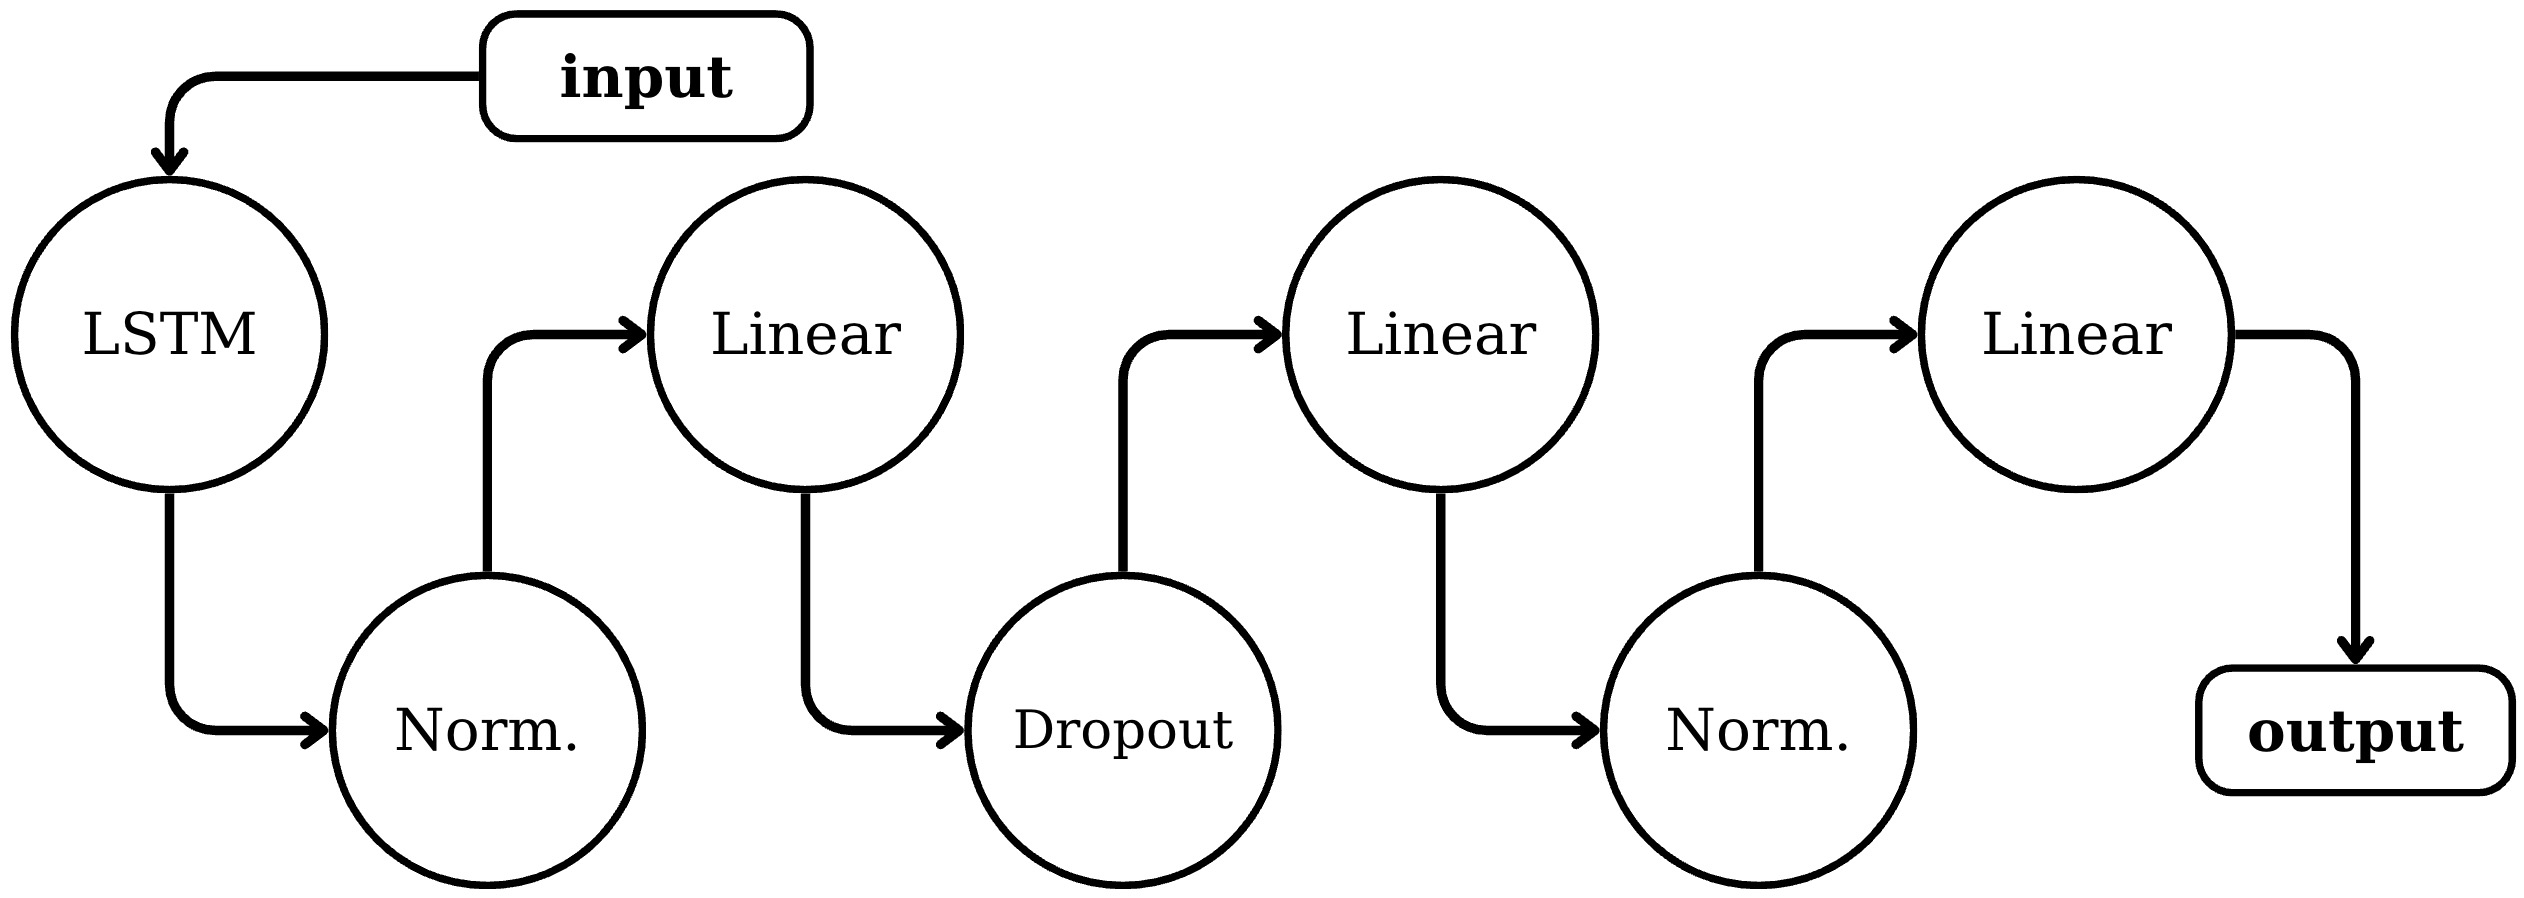
\includegraphics[width=0.65\textwidth]{images/gestor_arch.png}
    \caption{Arquitectura de la red neuronal DQN utilizada en el gestor de carga. Fuente: 
    Elaboración propia.}
    \label{fig:arch_dqn}
\end{figure}

\subsubsection{Entorno de la Red DQN-LSTM}
Para entrenar y evaluar el comportamiento del agente gestor, se ha desarrollado un entorno 
personalizado en Python~\cite{python2024language}. Este entorno representa un hogar con un vehículo 
eléctrico, y tiene en cuenta tanto el consumo energético no gestionable como la disponibilidad  del 
EV y el precio de la electricidad en cada intervalo de tiempo.

\paragraph{Estado del entorno.}
El vector de estado \(\mathbf{s}_t \in \mathbb{R}^8\) en cada instante \(t\) incluye las siguientes 
variables:
\begin{itemize}
    \item \textbf{State of Charge (SOC):} estado de carga actual del vehículo eléctrico, expresado 
    en kWh.
    \item \textbf{SOC objetivo:} nivel de carga deseado, también en kWh.
    \item \textbf{Hora normalizada:} instante del día en formato continuo \([-1, 1]\).
    \item \textbf{Consumo no gestionable (\(P_{NG}\)):} potencia usada por la vivienda que no se 
    puede desplazar.
    \item \textbf{Disponibilidad (\(A_t\)):} probabilidad de que el vehículo esté conectado en ese 
    instante.
    \item \textbf{Precio de la electricidad:} coste por kWh en el instante actual.
    \item \textbf{Media del precio de la electricidad:} media del precio de la electricidad en el 
    pasado reciente.
    \item \textbf{Desviación del precio de la electricidad:} diferencia entre el precio actual y su 
    media reciente, indicando si está por encima o por debajo del precio habitual.
\end{itemize}

\paragraph{Acciones.} 
La acción es binaria \(a_t \in \{0, 1\}\), indicando si se decide cargar (1) o no cargar (0) durante 
el intervalo actual de 15 minutos.

\paragraph{Dinámica.} 
Dado un estado y una acción, se debe calcular el nuevo estado del entorno, que desencadena dicha 
acción. Esto significa que el entorno debe calcular:
\begin{itemize}
    \item La potencia solicitada \(P = a_t \cdot P_{\text{max}}\).
    \item La energía cargada, ajustada a las restricciones físicas y de disponibilidad.
    \item La actualización del SOC: \(\Delta SOC = P \cdot \Delta t\), con 
    \(\Delta t = 0{,}25~\text{h}\).
    \item El coste de la carga en ese instante: \(C_t = P \cdot p(t)\).
    \item La recompensa obtenida, que depende de la acción tomada y del estado del entorno.
\end{itemize}

\paragraph{Función de recompensa.} 
La función de recompensa implementada tiene como objetivo guiar al agente hacia un comportamiento 
eficiente, seguro y económicamente óptimo. Para ello, combina penalizaciones por violar 
restricciones físicas o económicas, y recompensas por decisiones adecuadas en función del contexto 
del entorno. Esta función es una traducción literal de las restricciones impuestas en el 
optimizador clásico visto anteriormente.\\

En primer lugar, se penaliza el coste económico de la carga en cada instante de tiempo, calculado 
como \( C_t = P \cdot p(t) \), donde \(P\) es la potencia aplicada y \(p(t)\) el precio de la 
electricidad en el instante \(t\). Esta penalización incentiva al agente a cargar en momentos más 
baratos.\\

Además, se penaliza al agente en tres casos clave:
\begin{itemize}
    \item Cuando intenta cargar sin disponibilidad del vehículo (\(A_t = 0\)), se reduce la 
    recompensa con la energía desaprovechada.
    \item Cuando la potencia solicitada supera el margen disponible contratado con la red: \( P > P_{\text{red}} - P_{NG} \), 
    en cuyo caso se corrige la acción y se aplica de nuevo una penalización con el exceso.
    \item Cuando el SOC supera el valor objetivo fijado, o si se excede la capacidad de la batería.
    En este caso, se penaliza con lo que habría sido el coste incurrido en esta carga superflua.
\end{itemize}

Por otro lado, se añaden incentivos positivos en los siguientes casos:
\begin{itemize}
    \item Si el vehículo alcanza el SOC objetivo al final del día, se otorga una recompensa 
    adicional muy significativa (\(+50\)) para fomentar la planificación de largo plazo.
    \item Si se carga cuando la disponibilidad es alta y el SOC aún no ha alcanzado el objetivo, 
    se otorga una pequeña recompensa positiva para favorecer la acción oportuna.
    \item Toda energía cargada que se acerque al SOC deseado se premia con una recompensa 
    proporcional.
\end{itemize}

Finalmente, se penaliza ligeramente el hecho de no cargar cuando el vehículo está disponible y el 
SOC aún no ha alcanzado su nivel deseado. Esta penalización está diseñada para evitar que el 
agente se comporte demasiado conservador y desaproveche oportunidades de carga viables.\\

\paragraph{Formato del episodio.}  
Cada episodio simula un día completo dividido en intervalos de 15 minutos (96 pasos). El SOC se 
inicializa aleatoriamente entre 3\% y 25\% al inicio del día, y se va actualizando conforme a las 
decisiones del agente.

\subsubsection{Entrenamiento del Agente DQN-LSTM.}  
Durante el entrenamiento, el agente observa secuencias de estados \((s_{t-T}, \ldots, s_t)\) para 
estimar la utilidad esperada de ejecutar cada acción \(a \in \{0, 1\}\). La red neuronal devuelve 
dos valores, que serían la acción de cargar o no cargar el vehículo en el intervalo actual.

\paragraph{Representación temporal.}  
Para aportar contexto al momento de la carga, la disponibilidad y precio, de manera que no sea un 
análisis puntual de la situación, se utiliza una secuencia de entrada temporal de longitud 
\(T = 8\) pasos (2 horas), alimentada a través de la capa LSTM.

\paragraph{Parámetros del entrenamiento.}  
El entrenamiento se realiza durante \(N = 365\) episodios completos (días), con los siguientes 
hiperparámetros base:
\begin{itemize}
    \item \textbf{Tasa de aprendizaje (\(\alpha\))}: 0.001
    \item \textbf{Factor de descuento (\(\gamma\))}: 0.95
    \item \textbf{Exploración inicial (\(\epsilon\))}: 0.1, decreciendo progresivamente
    \item \textbf{Tamaño del batch}: 64
    \item \textbf{Tamaño de la secuencia temporal}: 8 pasos
    \item \textbf{Tamaño del buffer de experiencia}: 10000
\end{itemize}

Para la elección de los valores de estos hiperparámetros, se ha realizado un algoritmo de 
\textit{Grid Search} sobre un rango de valores, y se ha seleccionado el conjunto que mejor 
rendimiento ha obtenido en términos de recompensa media acumulada y estabilidad del aprendizaje.\\

Además, se emplea una política \(\epsilon\)-greedy, en la que el agente escoge acciones aleatorias 
con probabilidad \(\epsilon\) y sigue la política aprendida con probabilidad  \(1 - \epsilon\). El 
valor inicial de \(\epsilon\) se fija en 0.1, y se reduce progresivamente a lo largo de los 
episodios mediante una estrategia de decaimiento exponencial:

\begin{equation}
    \epsilon_t = \epsilon_{\text{min}} + (\epsilon_{\text{start}} - \epsilon_{\text{min}}) \cdot 
    e^{-\kappa t}
\end{equation}

con \(\epsilon_{\text{start}} = 0.1\), \(\epsilon_{\text{min}} = 0.05\), \(\kappa\)  una 
constante de decaimiento, y \(t\) el número de episodios transcurridos. Con esta estrategia, se 
busca que el agente sea mucho más "curioso" al comenzar el entrenamiento, explorando más 
posibilidades en el espacio de acciones, y vaya convergiendo progresivamente hacia las mejores 
políticas.

\paragraph{Algoritmo.}  
Se emplea el algoritmo clásico de \textit{Deep Q-Learning} con \textit{replay buffer}, que incluye 
actualizaciones periódicas de la red objetivo y política \(\epsilon\)-greedy. El error se calcula 
mediante pérdida MSE (\textit{Mean Squared Error}, Error Cuadrático Medio) entre la estimación del 
valor actual y el objetivo de Bellman, tal y como se ha presentado en el Capítulo~\ref{chapter:chapter2}.

\paragraph{Monitorización y métricas.}  
Durante el entrenamiento, se muestra una barra de progreso en terminal, y se registran métricas 
como recompensa promedio por episodio. También se exportan ficheros \texttt{.csv} de depuración con 
los valores de potencia aplicada, SOC, precio y recompensas en cada paso, permitiendo inspeccionar 
el comportamiento del agente en detalle.

\subsubsection{Resultados del Agente DQN-LSTM.}
Los resultados obtenidos por el agente gestor, después del entrenamiento, se muestran a continuación.
\begin{figure}[H]
    \centering
    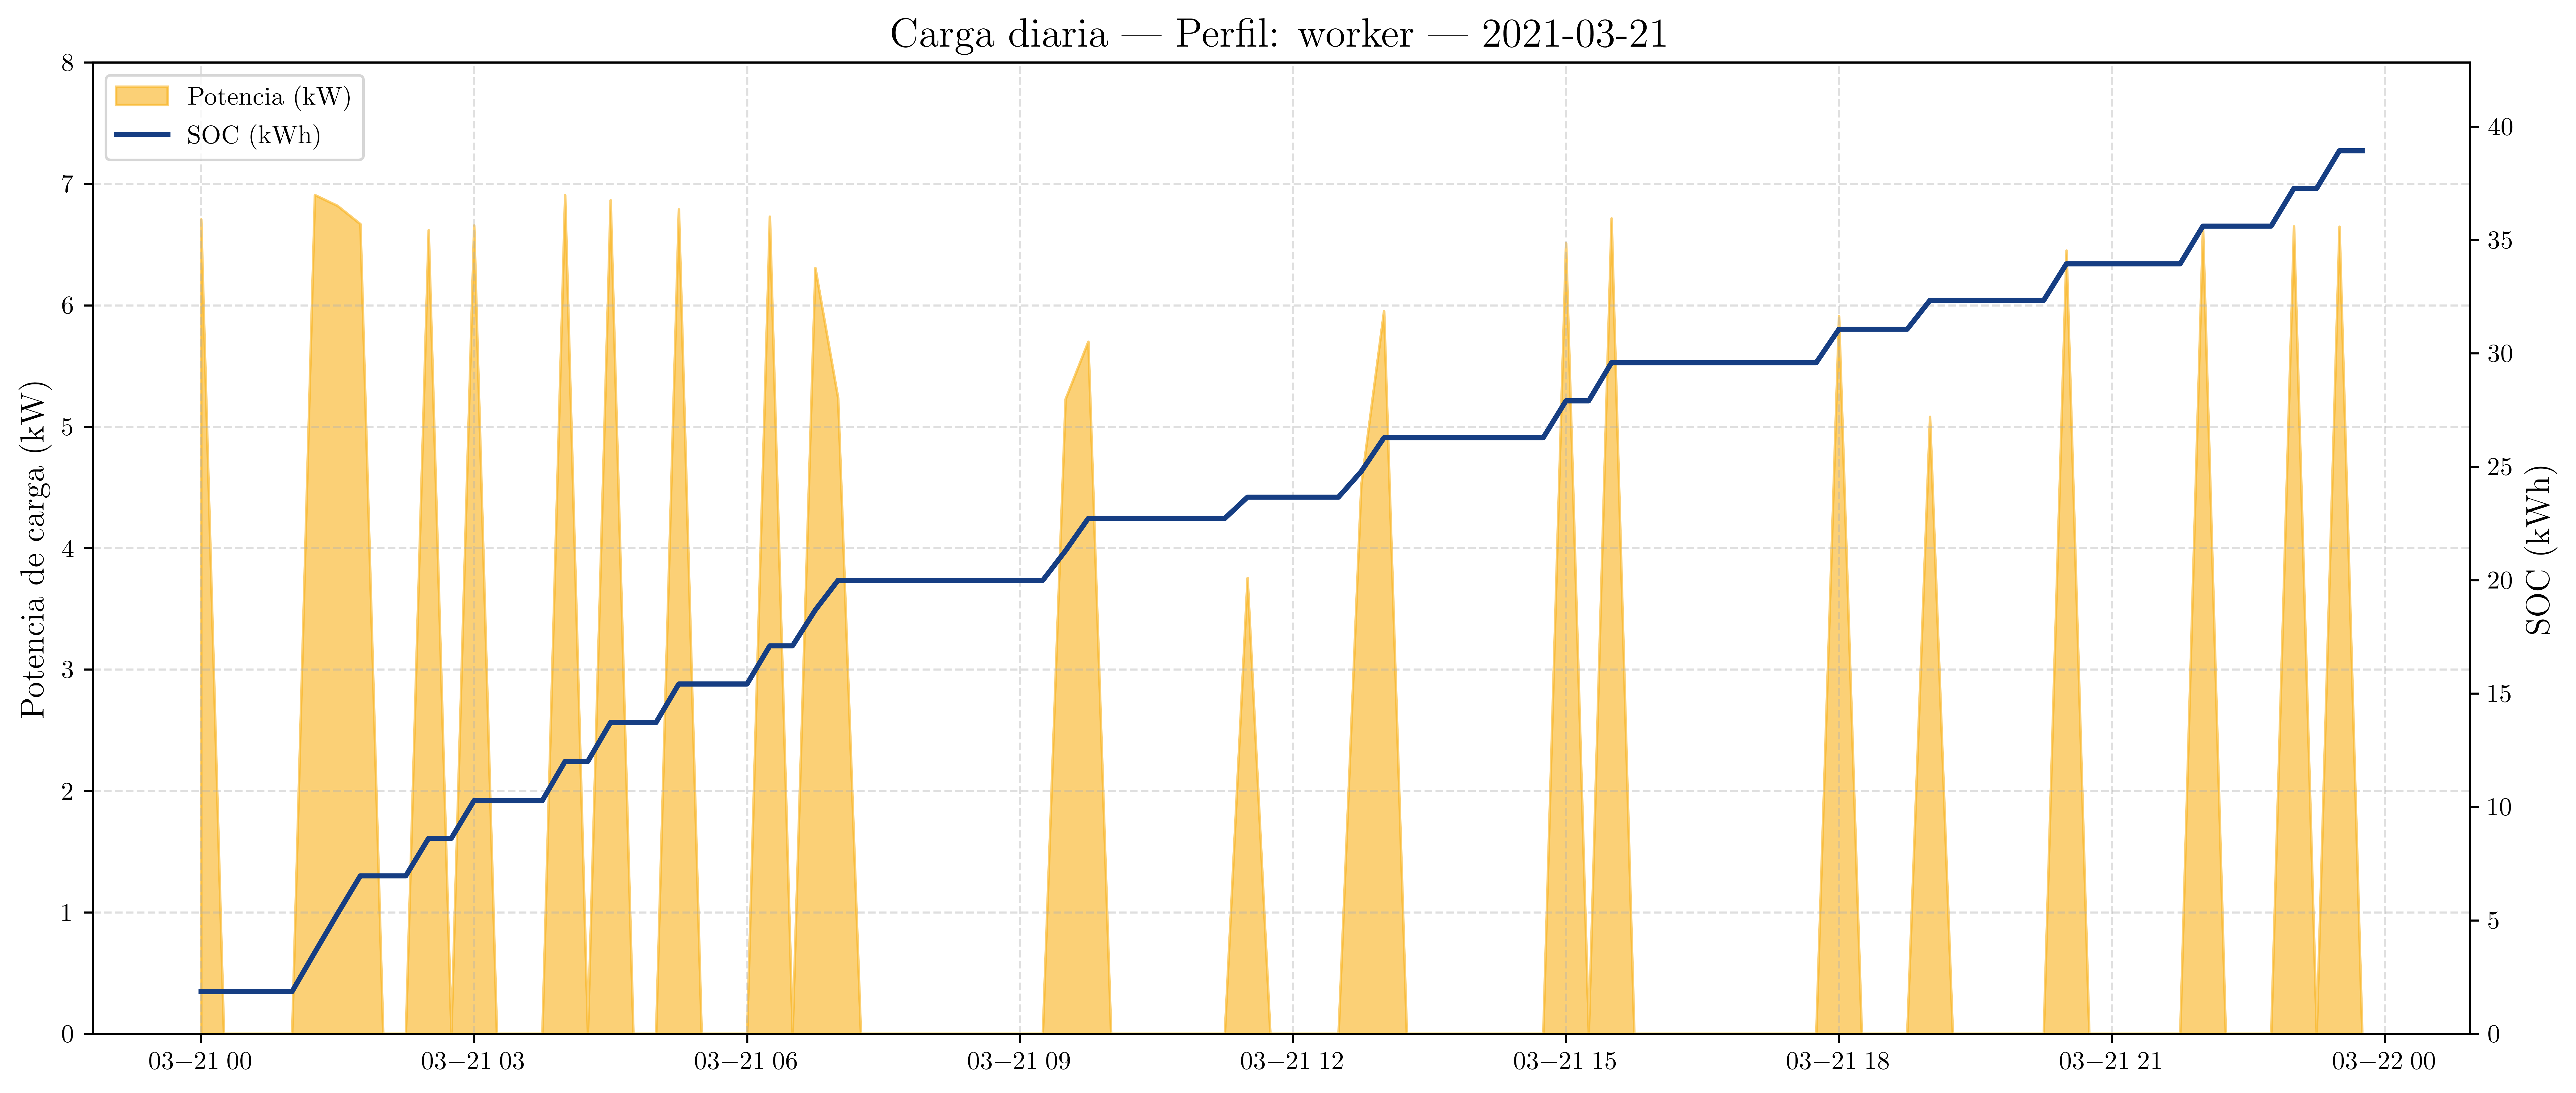
\includegraphics[width=0.7\textwidth]{images/dqnlstm/daily_behavior_2021-03-21_worker.png}
    \caption{Resultados del agente DQN-LSTM para el perfil \texttt{worker}: potencia aplicada y 
    evolución del SOC en un día. Fuente: Elaboración propia.}
    \label{fig:dqn_daily_profiles}
\end{figure}
\begin{figure}[H]
    \centering
    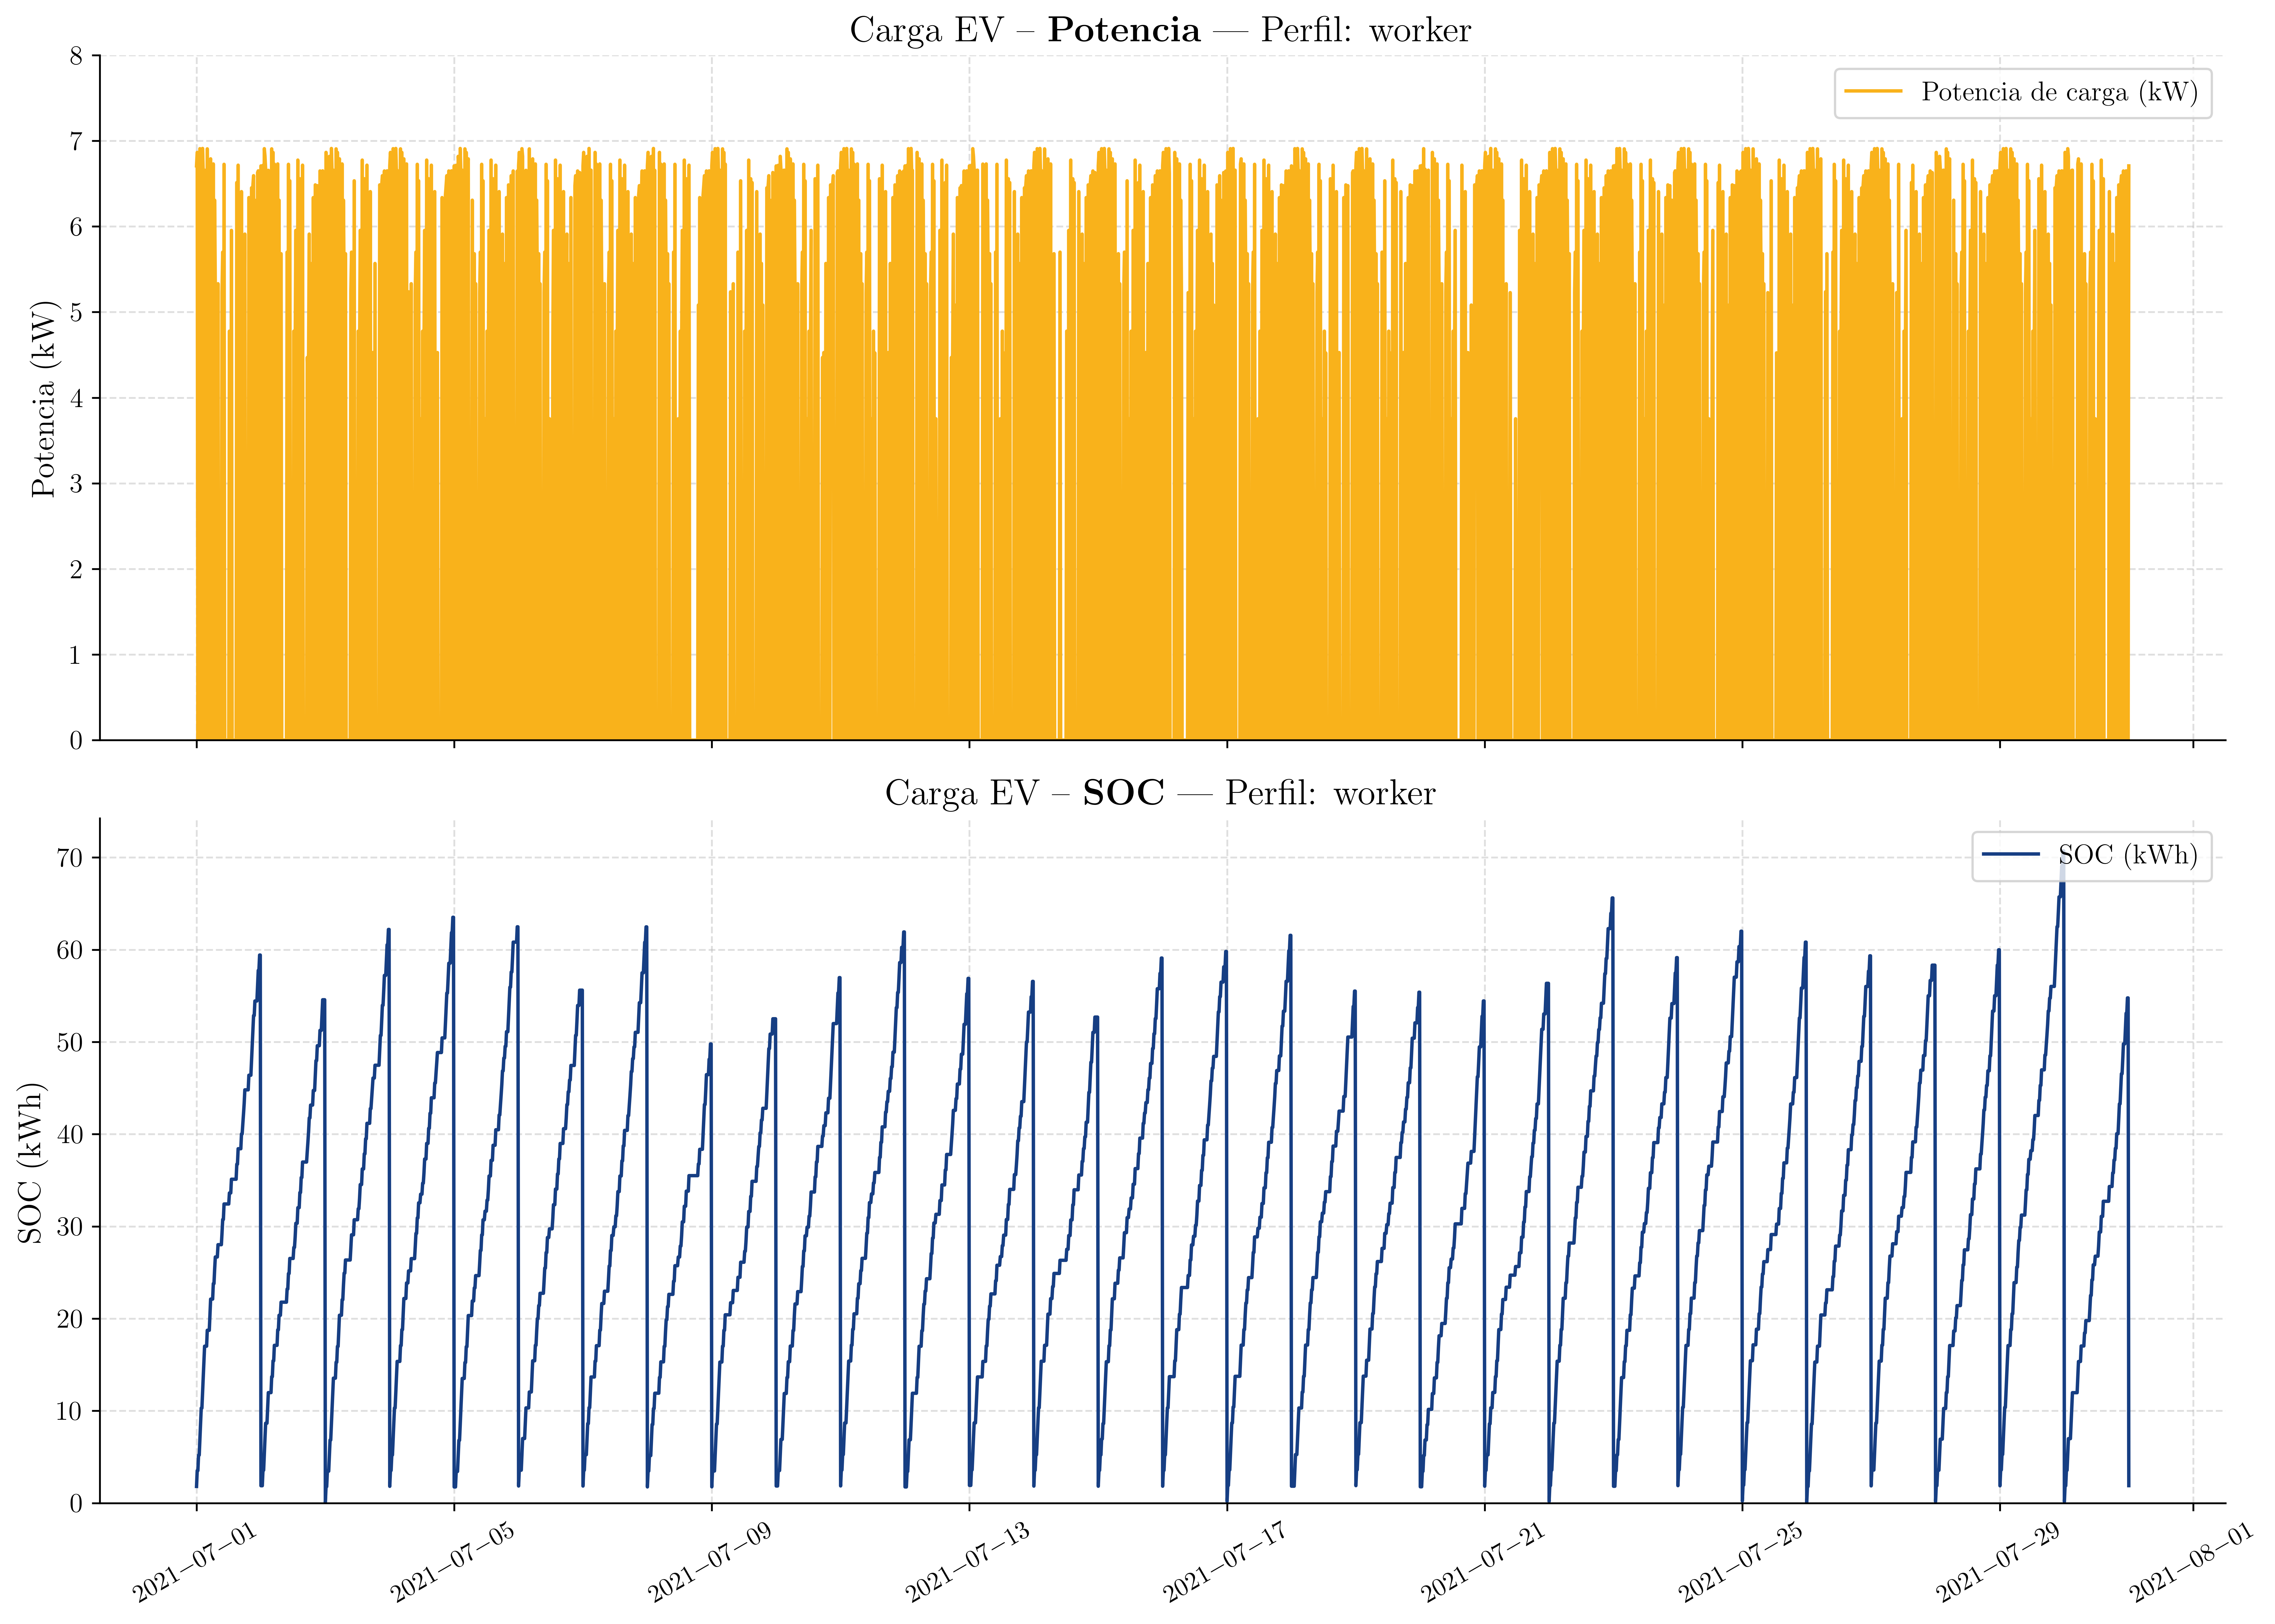
\includegraphics[width=0.7\textwidth]{images/dqnlstm/worker_monthly_behavior_july_bold.png}
    \caption{Resultados del agente DQN-LSTM para el perfil \texttt{worker}: potencia aplicada y 
    evolución del SOC a lo largo de un mes. Fuente: Elaboración propia.}
    \label{fig:dqn_global_profiles}
\end{figure}

Igual que con el optimizador clásico, la Figura~\ref{fig:dqn_daily_profiles} muestra el
comportamiento diario del agente gestor para el perfil \texttt{worker}, donde se observa la
evolución de la potencia entregada al cargador y la evolución del estado de carga (SOC) del
vehículo eléctrico a lo largo del día. Por otro lado, la Figura~\ref{fig:dqn_global_profiles}
muestra las mismas variables pero a lo largo de un mes entero, donde se puede observar las
tendencias de carga y consumo del vehículo eléctrico a lo largo de todo el mes.\\

La red neuronal DQN-LSTM ha aprendido a gestionar la carga del vehículo eléctrico de forma
eficiente, adaptándose a las condiciones del entorno y optimizando el coste de la carga. La 
intencionalidad de la carga es aparente en ambas gráficas, ya que el gestor ha entendido qué 
momentos del día son los más adecuados para cargar el EV, teniendo en cuenta la variabilidad de la 
disponibilidad del propio vehículo para la carga, el precio de la electricidad, y demás variables
del entorno.\\

Los incentivos de carga implanatados en el entorno, al igual que los "castigos" por mostrar 
comportamientos no deseados o subóptimos, han ayudado al agente a tomar mejores decisiones, y más
informadas a lo largo del tiempo. Por ejemplo, se puede observar cómo el agente ha aprendido a
cargar el vehículo eléctrico durante la noche, cuando la disponibilidad es alta y el precio de la
electricidad es más bajo, y a evitar cargar durante el día, en los intervalos en que el consumo 
energético sería más costoso para el cliente.\\

Además, se puede observar el funcionamiento de las restricciones impuestas en el entorno, si se 
presta atención a la potencia entregada al cargador durante el día, concretamente sobre las 12-13h, 
donde el agente gestor ha moderado la potencia entregada al cargador, ya que el consumo energético 
de la vivienda es más alto, y por tanto, la potencia disponible para cargar el vehículo eléctrico 
es menor.\\

Con una vista mensual, a medio plazo, el comportamiento estable y positivo de la red se mantiene y
se pone de manifiesto. La tendencia de carga del EV para este perfil se mantiene, cargando pronto
e intentando llegar al SOC objetivo - el 80\% de la capacidad de la batería, por diseño - antes de
que termine el día. Además, se observa que el agente gestor ha aprendido a adaptarse a las
variaciones del precio de la electricidad, cargando en los momentos más económicos y evitando
cargas innecesarias en momentos de precios altos.\\

De nuevo, como con el optimizador clásico, se muestra únicamente el perfil \texttt{worker} como
ejemplo más representativo, ya que sería el perfil de consumo energético más habitual. Los
resultados y visualizaciones adicionales tanto para este perfil como para los demás se pueden
encontrar en el anexo~\ref{appendix:appendixA}.\\

Finalmente, se han extraído métricas y resultados adicionales obtenidos tras el entrenamiento y 
pruebas del agente gestor, para evaluar su rendimiento en la gestión de la carga del vehículo
léctrico. Estos resultados se muestran a continuación:
\begin{table}[H]
    \centering
    \begin{tabular}{lccc}
            \textbf{Perfil} & $\overline{\text{Coste}}$ (EUR) & $\overline{\text{Energía}}$ (kWh) & Eficiencia(kWh/EUR) \\
        \midrule
        worker      & 5,04  & 209,68 & 41,63 \\
        flexible    & 2,93  & 120,07 & 40,33 \\
        retired     & 1,64  & 63,28  & 37,14 \\
        traveller   & 7,09  & 325,07 & 45,93 \\
        night\_owl  & 6,21  & 268,06 & 43,07 \\
        \bottomrule
    \end{tabular}
    \caption{Resumen de métricas diarias por perfil para el agente DQN-LSTM.}
    \label{tab:metrics_dqn_summary}
\end{table}

El rendimiento computacional de la red también ha sido registrado durante el entrenamiento y las 
pruebas, y los tiempos obtenidos son los siguientes:
\subsubsection{Métricas computacionales}
A continuación se presentan los tiempos de entrenamiento e inferencia obtenidos para cada perfil durante el entrenamiento y pruebas del agente DQN-LSTM:

\begin{table}[H]
    \centering
    \begin{tabular}{lcc}
        \toprule
        \textbf{Perfil} & \textbf{Tiempo total train (min)} & \textbf{\(\overline{\text{Tiempo de inferencia}}\) (ms)} \\
        \midrule
        worker      & 3.98 & 0.174 \\
        flexible    & 4.39 & 0.294 \\
        retired     & 4.29 & 0.301 \\
        traveller   & 4.45 & 0.309 \\
        night\_owl  & 4.37 & 0.306 \\
        \bottomrule
    \end{tabular}
    \caption{Tiempos de entrenamiento e inferencia por perfil para el agente DQN-LSTM.}
\end{table}

El tiempo medio de entrenamiento por perfil es relativamente bajo, 4.17 minutos por perfil, lo que 
indica que el agente DQN-LSTM es capaz de aprender de forma eficiente a partir de los datos 
recibidos. Además, y más importante aún, el tiempo medio de inferencia es muy bajo, con una media 
de 0.252 milisegundos por perfil, alcanzando un mínimo de tan solo 174 milisegundos de media si el perfil es 
\texttt{worker}. Esto indica que el agente es capaz de tomar decisiones en tiempo real, lo que es 
esencial para la gestión eficiente de la carga del vehículo eléctrico.\\

Además, con unos tiempos de inferencia tan reducidos, una posible implementación en hardware de 
este gestor no requeriría de mucha potencia computacional, sino tan solo para el entrenamiento.